% GENERATED by `python -m bench.figures --write` from
% bench/results/adversary.json. Do not edit: `--check` runs in CI and
% fails if this file and the committed runs disagree.
\begin{figure}[t]
\centering
  \begin{subfigure}[t]{0.48\textwidth}
  \centering
  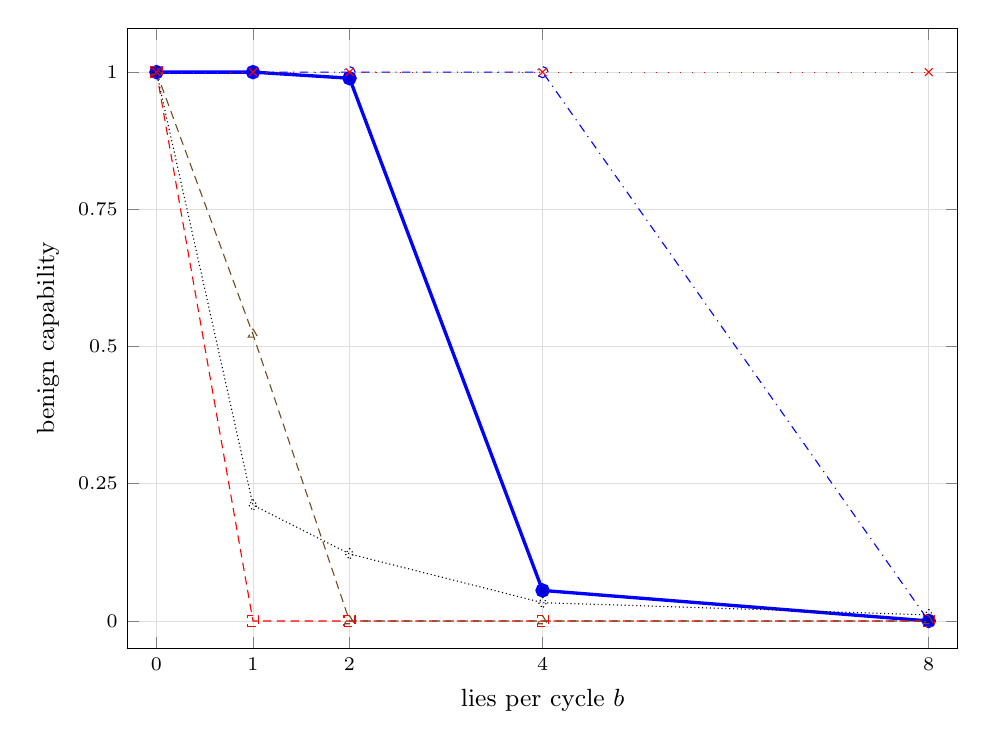
\begin{tikzpicture}
    \begin{axis}[
      width=\textwidth, height=0.78\textwidth,
      xlabel={lies per cycle $b$}, ylabel={benign capability},
      xmin=-0.3, xmax=8.3, ymin=-0.05, ymax=1.08,
      xtick={0,1,2,4,8}, ytick={0,0.25,0.5,0.75,1},
      tick label style={font=\scriptsize},
      label style={font=\small},
      grid=major, grid style={very thin, gray!25},
      legend style={font=\scriptsize, legend columns=3, draw=none},
      legend to name=adversarylegend,
    ]
      \addplot+[very thick, mark=*] coordinates {(0,1.0000) (1,1.0000) (2,0.9889) (4,0.0556) (8,0.0000)};
      \addlegendentry{ledger}
      \addplot+[mark=square, densely dashed] coordinates {(0,1.0000) (1,0.0000) (2,0.0000) (4,0.0000) (8,0.0000)};
      \addlegendentry{evict-on-negative}
      \addplot+[mark=triangle, densely dashed] coordinates {(0,1.0000) (1,0.5222) (2,0.0000) (4,0.0000) (8,0.0000)};
      \addlegendentry{consecutive $k{=}2$}
      \addplot+[mark=diamond, densely dotted] coordinates {(0,1.0000) (1,0.2111) (2,0.1222) (4,0.0333) (8,0.0111)};
      \addlegendentry{quarantine $m{=}3$}
      \addplot+[mark=o, dashdotted] coordinates {(0,1.0000) (1,1.0000) (2,1.0000) (4,1.0000) (8,0.0000)};
      \addlegendentry{bandit}
      \addplot+[mark=x, loosely dotted] coordinates {(0,1.0000) (1,1.0000) (2,1.0000) (4,1.0000) (8,1.0000)};
      \addlegendentry{keep everything}
    \end{axis}
  \end{tikzpicture}
  \caption{benign capability retained}
  \end{subfigure}
  \hfill
  \begin{subfigure}[t]{0.48\textwidth}
  \centering
  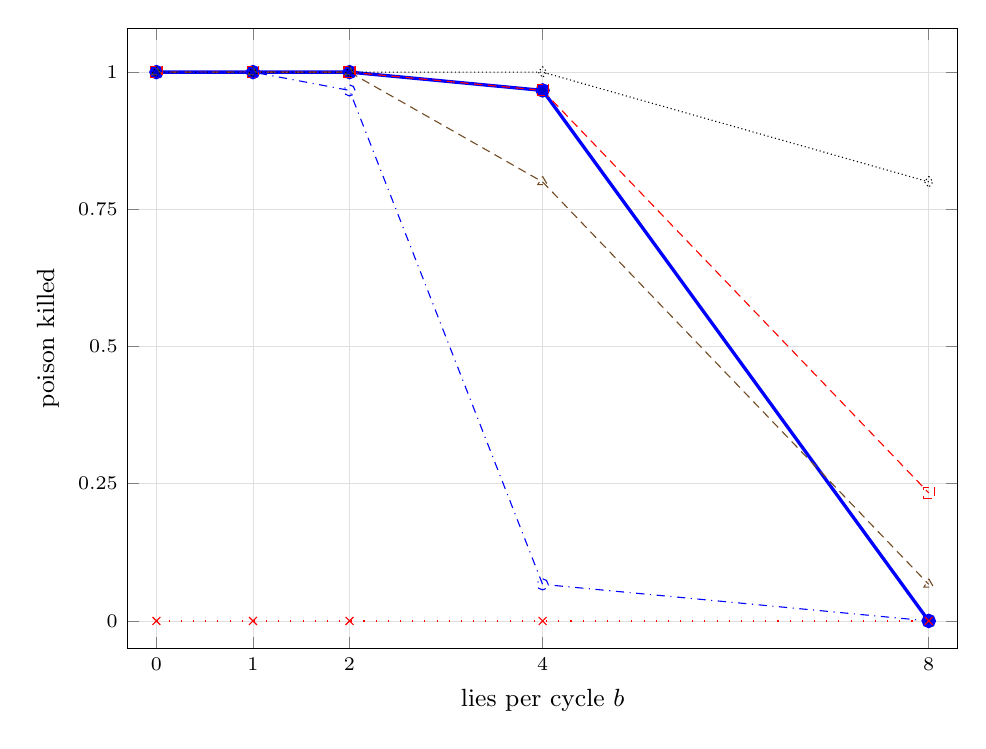
\begin{tikzpicture}
    \begin{axis}[
      width=\textwidth, height=0.78\textwidth,
      xlabel={lies per cycle $b$}, ylabel={poison killed},
      xmin=-0.3, xmax=8.3, ymin=-0.05, ymax=1.08,
      xtick={0,1,2,4,8}, ytick={0,0.25,0.5,0.75,1},
      tick label style={font=\scriptsize},
      label style={font=\small},
      grid=major, grid style={very thin, gray!25},
    ]
      \addplot+[very thick, mark=*] coordinates {(0,1.0000) (1,1.0000) (2,1.0000) (4,0.9667) (8,0.0000)};
      \addplot+[mark=square, densely dashed] coordinates {(0,1.0000) (1,1.0000) (2,1.0000) (4,0.9667) (8,0.2333)};
      \addplot+[mark=triangle, densely dashed] coordinates {(0,1.0000) (1,1.0000) (2,1.0000) (4,0.8000) (8,0.0667)};
      \addplot+[mark=diamond, densely dotted] coordinates {(0,1.0000) (1,1.0000) (2,1.0000) (4,1.0000) (8,0.8000)};
      \addplot+[mark=o, dashdotted] coordinates {(0,1.0000) (1,1.0000) (2,0.9667) (4,0.0667) (8,0.0000)};
      \addplot+[mark=x, loosely dotted] coordinates {(0,0.0000) (1,0.0000) (2,0.0000) (4,0.0000) (8,0.0000)};
    \end{axis}
  \end{tikzpicture}
  \caption{poison-kill rate}
  \end{subfigure}

  \par\vspace{0.8em}
  \pgfplotslegendfromname{adversarylegend}
\caption{The curation-targeted adversary, 30 seeds, plotted as the two
halves the result has to be read in. \emph{Left}: benign capability
retained. \emph{Right}: poison-kill rate. The counters fall on the left
panel by $b{=}1$, which is the separation the paper is about. The figure
exists for the other half: \texttt{keep\_everything} traces a flat
$1.00$ across the left panel and a flat $0.00$ across the right, and the
bandit holds the left panel to $b{=}4$ while giving the right one away.
A perfect capability score beside a zero defence score is abstention, not
defence, and either panel alone hides it. Only the ledger holds both, and
only to its published boundary between $b{=}2$ and $b{=}4$. Generated
from committed per-seed data by \texttt{bench/figures.py}; CI fails if
the two disagree.}
\label{fig:adversary}
\end{figure}
